\documentclass[12pt]{article}
\author{Alex Ho}
\title{AST5220 - Cosmology 2 \\ Milestone 2}
\usepackage{listings}
\usepackage{graphicx}
\usepackage{verbatim}
\usepackage{amsmath}
\usepackage{float}
\usepackage[utf8]{inputenc}
\usepackage{xcolor}
\usepackage{booktabs}
\usepackage{hyperref}
\usepackage{placeins}
\usepackage{parskip}
\setlength\parskip{\baselineskip}
\setlength\parindent{0pt}

\lstset{
language=Python,
basicstyle=\ttfamily,
otherkeywords={__init__},             
keywordstyle=\ttfamily\color{blue!90!black},
keywords=[2]{True,False},
keywordstyle={[2]\ttfamily\color{red!40!black}},
emph={MyClass,class, def},          
emphstyle=\ttfamily\color{red!83!black},    
stringstyle=\color{green!45!black},
showstringspaces=false,
commentstyle=\color{magenta},
breaklines=true,
tabsize=3,
moredelim=**[is][\color{blue}]{@}{@}
}
\begin{document}
\maketitle
The program, plots and the report can be found in the following Github page:

\url{https://github.com/AHo94/AST5220_Projects/tree/master/Project2}
\subsection*{Mathematics}
We start with the differential equation of the optical depth, given as
\begin{align}
\frac{d\tau}{dx} = -\frac{n_e \sigma_T a}{\mathcal{H}} = -\frac{n_e \sigma_T}{H}
\end{align}
Where $\sigma_T$ is the Thompson cross-section, $H$ the Hubble parameter and $n_e$ the number density for free electrons. To compute the electron density, we define the fractional electron density $X_e \equiv n_e/n_H$. $X_e$ can be found in two different ways
\subsection*{Physical dimensions}
\subsubsection*{Saha equation}
One way to determine $X_e$ is by using the Saha equation. The Saha equation is a good approximation if $X_e \approx 1$, that is, for early times of the universe. Saha equation is given as
\begin{align}
\frac{X_e^2}{1-X_e} = \frac{1}{n_b}\left( \frac{m_e T_b}{2\pi}\right)^{3/2}e^{-\epsilon_0/T_b}
\end{align}
First thing to note is that the left hand side is dimensionless, whereas the right hand side has the dimension $(\text{kg K})^{3/2}\text{m}^3$ and the argument inside the exponential (which should be dimensionless) has the dimension $\text{J}/\text{K}$. We want to multiply a certain combination of $c, \hbar$ or $k_b$ to turn the right hand side dimensionless. Testing this for different combinations, we get the Saha equation in dimensionless form
\begin{align}
\frac{X_e^2}{1-X_e} =\frac{1}{n_b}\left( \frac{m_e T_b k_b}{2\pi \hbar^2}\right)^{3/2}e^{-\epsilon_0/(k_b T_b)}
\end{align}
This can be written in the form
\begin{align}
X_e^2 + BX_e - B = 0, \quad \text{where } B = \frac{1}{n_b}\left( \frac{m_e T_b k_b}{2\pi \hbar^2}\right)^{3/2}e^{-\epsilon_0/(k_b T_b)}
\end{align}
This is just a second order equation, which can be easily solved.
\subsubsection*{Peebles' equation}
The second way to determine $X_e$ is to use Peebles' equation. It is a good approximation when $X_e \ll 1$. Peebles' equation is given as
\begin{align}
\frac{dX_e}{dx} = \frac{C_r(T_b)}{H}\left[\beta(T_b)(1-X_e) - n_H \alpha^{(2)}(T_b)X_e^2\right]
\end{align}
This depends on many other parameters, which I will for now not write down. Once again, the left hand side is dimensionless, but the right hand side has the dimension of seconds, due to the Hubble parameter. The tricky part now is to determine whether $C_r(T_b)$ or $\beta(T_b)$ (and $\alpha^{(2)}(T_b)$) are dimensionless parameters. Let us first check $C_r(T_b)$, which is given as
\begin{align}
C_r(T_b) = \frac{\Lambda_{2s\to 1s} + \Lambda_{\alpha}}{\Lambda_{2s\to 1s}+ \Lambda_\alpha + \beta^{(2)}(T_b)}
\end{align}
Where $\Lambda_{2s\to 1s} = 8.227s^{-1}$, i.e has the unit of $s^{-1}$. This parameter appears both on the numerator and the denominator, which implies that $C_r(T_b)$ is dimensionless. Now we have to determine the dimensions of $\Lambda_\alpha$ and $\beta^{(2)}(T_b)$. Looking at the numerator of $C_r(T_b)$, we demand that $\Lambda_\alpha$ has to have dimension of $s^{-1}$ as well, which ensures that we add two of physical quantities of same dimension \footnote{Let's be honest here. Adding, for instance, $1$kg and $1$m does not make much sense.}. Currently, $\Lambda_\alpha$ is given as
\begin{align}
\Lambda_\alpha = H \frac{(3\epsilon_0)^3}{(8\pi)^2n_{1s}}
\end{align}
which currently has the dimension $\text{J}^3\text{m}^{-3}\text{s}^{-1}$. To fix this, we can multiply with $1/(\hbar c)^3$, so the fixed quantity becomes
\begin{align}
\Lambda_\alpha = H\frac{(3\epsilon_0)^3}{(8\pi)^2n_{1s}}\left(\frac{1}{\hbar c}\right)^3
\end{align}
Same reasoning can be applied to $\beta^{(2)}(T_b)$. I will not go into much detail here, but the parameters that are fixed, with respect to their dimensions, are the following:
\begin{align}
\beta^{(2)}(T_b) &= \beta(T_b)e^{3\epsilon_0/(4k_bT_b)}\\
\beta(T_b) &= \alpha^{(2)}(T_b)\frac{k_b^{3/2}}{\hbar^3}\left(\frac{m_e T_b}{2\pi} \right)^{3/2}e^{-\epsilon_0/(k_b T_b)}\\
\alpha^{(2)}(T_b) &= \frac{64\pi}{\sqrt{27\pi}}\frac{\alpha^2}{m_e^2} \frac{\hbar^2}{c} \sqrt{\frac{\epsilon_0}{k_b T_b}}\phi_2(T_b) \\
\phi_2(T_b)&= 0.448\ln[\epsilon_0/(k_b T_b)]
\end{align}
Peebles' equation itself remains unchanged.
\subsubsection*{The optical depth}
The right hand side of equation (1) has the dimension s m$^{-1}$. We want the optical depth to be dimensionless so that the visibility function $g(x)$ (as well as the exponential in  $g(x)$) remains dimensionless. This is easily fixed by multiplying with $c$ on the right hand side, that is
\begin{align}
\frac{d\tau}{dx} = -\frac{n_e \sigma_T c}{H}
\end{align}
\subsection*{Numerics}
\subsubsection*{Overflows in Peebles' equation}
When we do the computation of the Peebles' equation, we will quickly run into overflow problems. This is especially true in the $\beta^{(2)}(T_b)$ term, where the exponential explodes because $\epsilon_0/(k_bT_b)$ is of order $\sim 10^4$. Instead, we can write out the expression of $\beta^{(2)}(T_b)$ to include the exponential in $\beta(T_b)$, which we write into a single exponential. That is
\begin{align}
\beta^{(2)}(T_b) &= \alpha^{(2)}(T_b)\frac{k_b^{3/2}}{\hbar^3}\left(\frac{m_e T_b}{2\pi}\right)^{3/2}e^{-\epsilon_0/(k_bT_b)}e^{3\epsilon_0/(4k_bT_b)} \nonumber \\
&= \alpha^{(2)}(T_b)\frac{k_b^{3/2}}{\hbar^3}\left(\frac{m_e T_b}{2\pi}\right)^{3/2}e^{-\epsilon_0/(4k_bT_b)}
\end{align}
The exponential should now no longer give any problems with overflows.
\subsubsection*{The program}
The program is a continuation of the program from the previous milestone, with some extras and small changes to the old code. 

The function \verb|Get_eta| has been replaced with a new function \verb|Cubic_spline|, which does the exact same thing, but applies for any function $f(x)$. The function \verb|Spline_DoubleDerivative|, from milestone 1, has also been replaced with a new function, \verb|Spline_derivative|, which applies to any derivatives and also uses natural spline boundary condition. Like the previous milestone, the interpolation is done by using Scipy's \verb|interpolate| functions.

Calculating $X_e$ is done in its own function \verb|Calculate_Xe|. We assume $X_e = 1$ as the initial condition. The Saha equation and Peebles' equation has also been split into two functions. When solving Saha equation, we assume that the second order equation takes the form $X_e^2 + BX_e - B = 0$. From this, we use Numpy's function \verb|roots| to solve this second order equation and returns the positively valued $X_e$. Peebles' equation is solved as a first order differential equation, using Scipy's \verb|odeint| function, and the initial condition of $X_e$ is the last calculated $X_e$ value from the Saha equation. Both these methods has a lot of constant terms which can be pre-calculated outside the loops (calculated as global constants), which will reduce the overall computation time.

Once we have calculated $X_e$, we can compute $n_e = X_e n_H$. Note that the number density of the electrons is a function of $x$, that is $n_e = n_e(x)$. Each value of $n_e$ thus have their corresponding value of $x$. We have to keep this in mind when calculating $\tau$. We only know the initial condition of $\tau$, which is $\tau(0) = 0$, i.e, zero today. Because of this, we will have to solve $\tau$ ''backwards'' in time, so we will have to assign a new array for $x$, which we call \verb|x_tau|. This array is the same as \verb|x_eta|, but in reverse order. While calculating $\tau$, we will have to find the $n_e$ value, which corresponds to the correct $x$ value. The calculated $\tau$ array is now in reversed order, with respect to \verb|x_eta|, so we will have to reverse the whole array before we calculate the visibility function.

When we have calculated $\tau$, again using Scipy's \verb|odeint|, we can calculate the visibility function $\tilde{g} = -\tau'\exp(-\tau)$. Note that $\tau'$ is the interpolated values of $\tau$, and not the one from equation (13). The interpolated values are calculated using the spline functions, explained above. With the interpolated values of $\tau'$ and computed values of $\tau$, we use the function \verb|Visibility_func| to compute $\tilde{g}$. The number of points \verb|n_eta| has been increased from 1000 to 3000 to give a better resolution to the visibility function. However, too many points will give some instabilities (for unknown reasons) to both $\tau'$ and $\tau''$.

All sanity checks are done with respect to the results from  Callin, in reference [1].
\subsection*{Plots}
\begin{figure}[H]
\centering
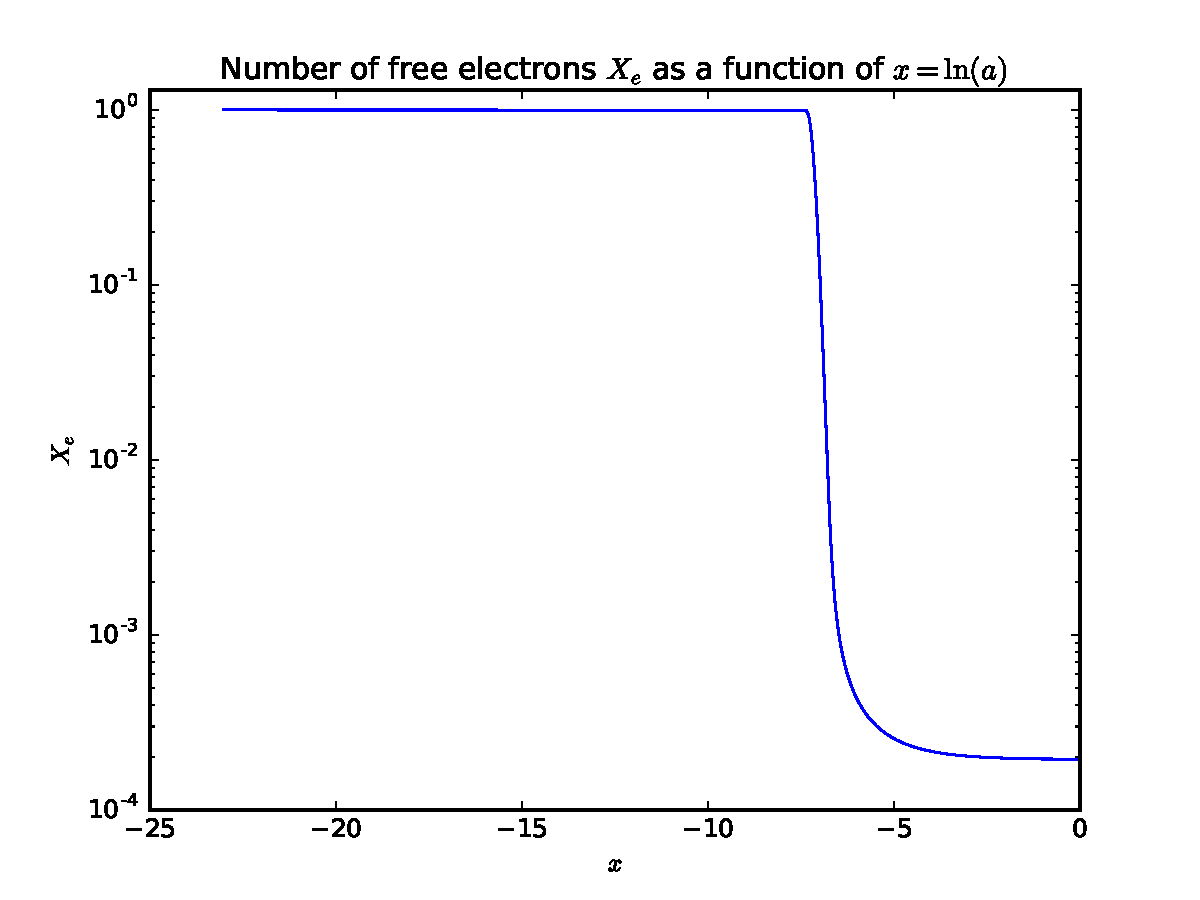
\includegraphics[width=0.75\linewidth]{Plots/ElectronNumber.pdf}
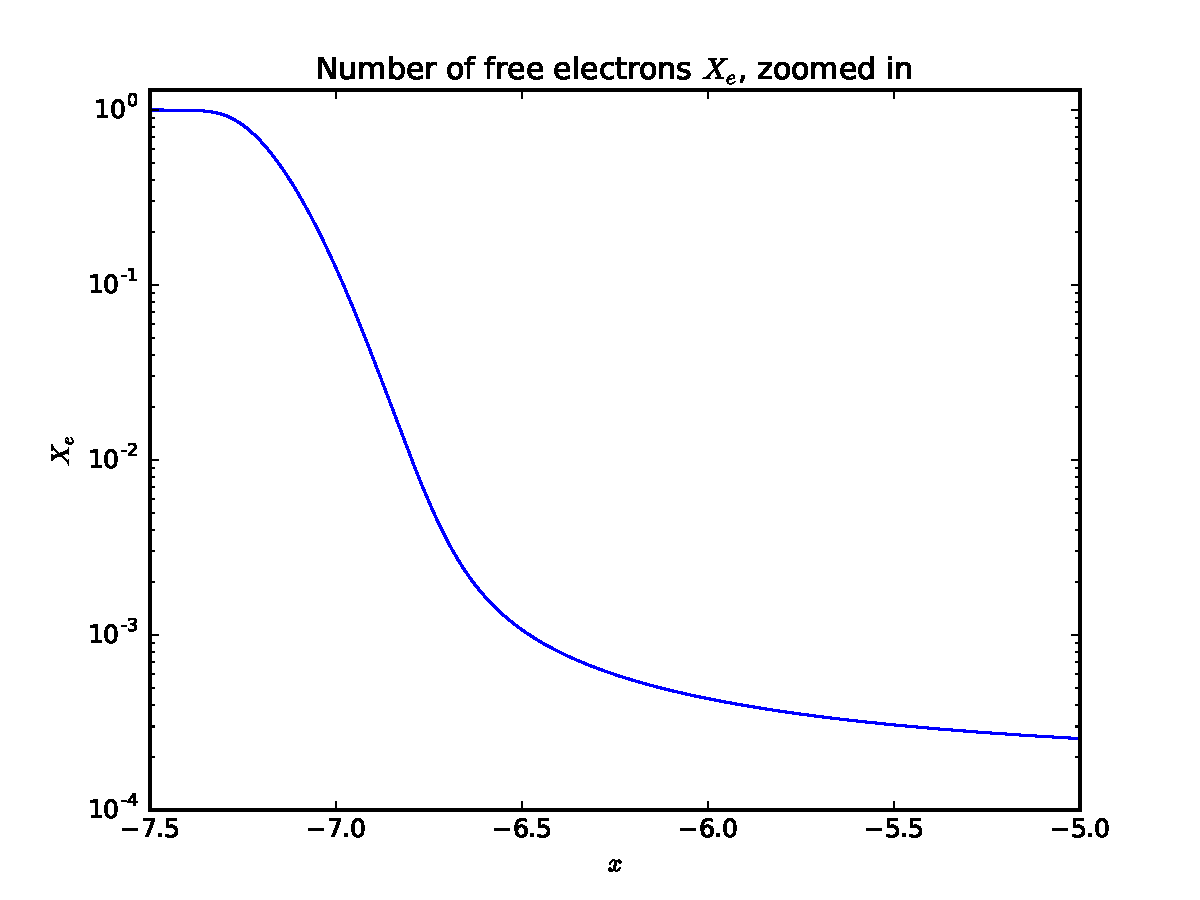
\includegraphics[width=0.75\linewidth]{Plots/ElectronNumberZoomed.pdf}
\caption{The number of free electrons as a function of $x=\ln a$. The bottom image is a zoomed in segment from $x=-7.5$ to $x=-5$ and it serves as a sanity check with respect to figure 1 in Callin. Although, we were asked to plot it as a function of $z$, I decided to plot it as a function of $x$ because an array for $z$, with $a_{init}=10^{-10}$ to $a=1$ would be very hard to scale with 3000 points.}
\end{figure}

%\begin{figure}[H]
%\centering
%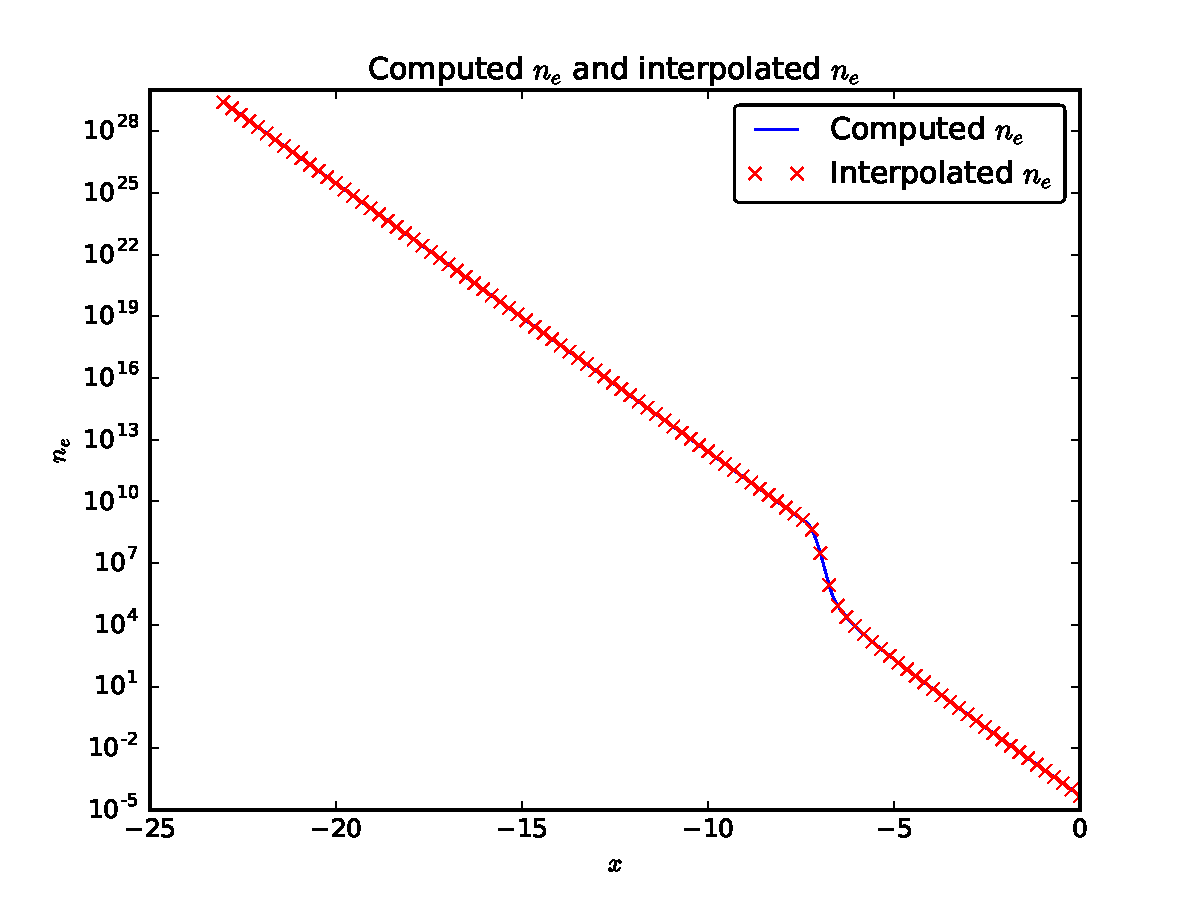
\includegraphics[width=\linewidth]{Plots/InterpolatedElectronDensity.pdf}
%\caption{Plot of the number density of the electrons. This plot also serves as a sanity check of the interpolation, to see whether it works or not. We see that the interpolation does its job quite nicely. The interpolated segment is in the time when recombination started to the end of recombination.}
%\end{figure} 

\begin{figure}[H]
\centering
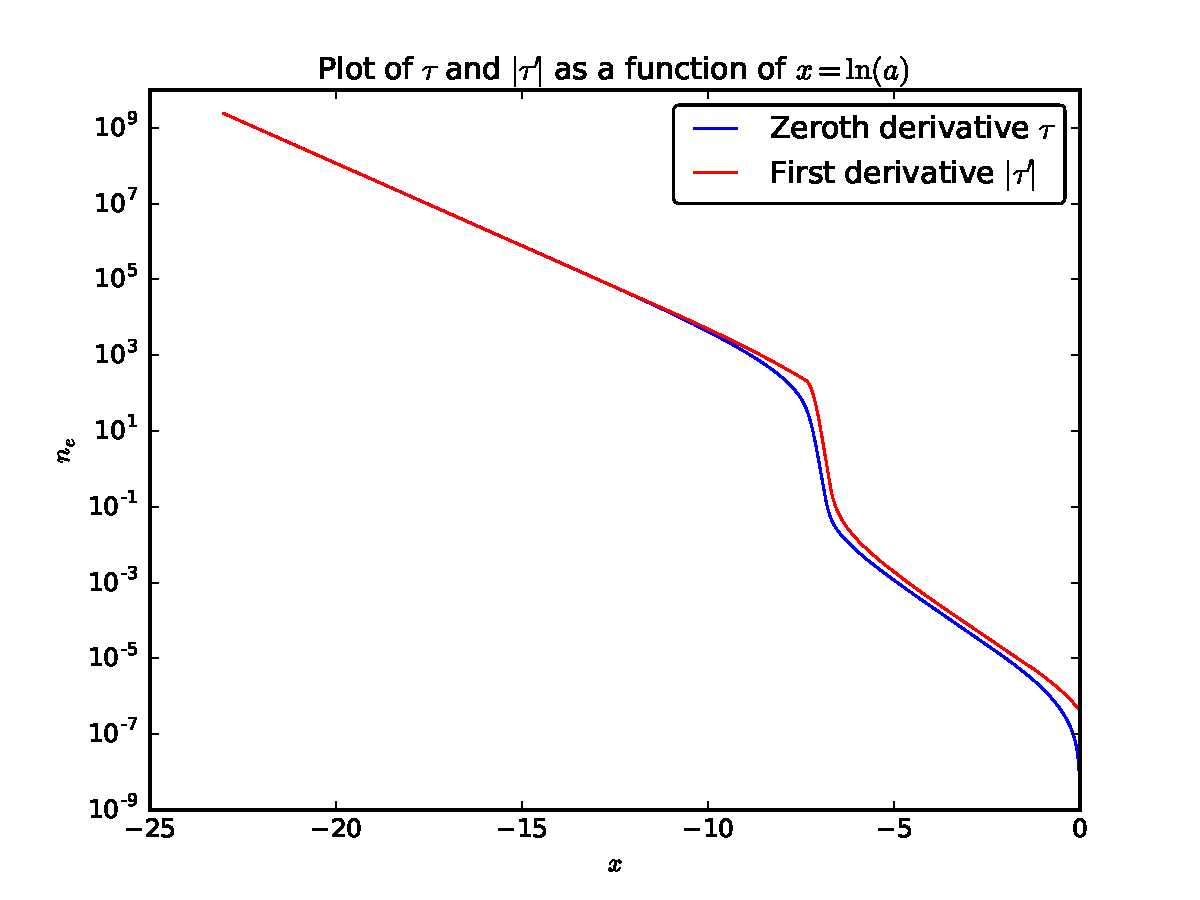
\includegraphics[width=\linewidth]{Plots/FirstDerivativeTau.pdf}
\caption{Plot of the computed optical depth $\tau$  (blue),  its interpolated derivative $|\tau'|$ (red) and the interpolated second derivative $|\tau''|$. The number of interpolated points for the second derivative was reduced from 3000 to 200, due to the instabilities it caused (as seen in the figure).}
\end{figure}

\begin{figure}[H]
\centering
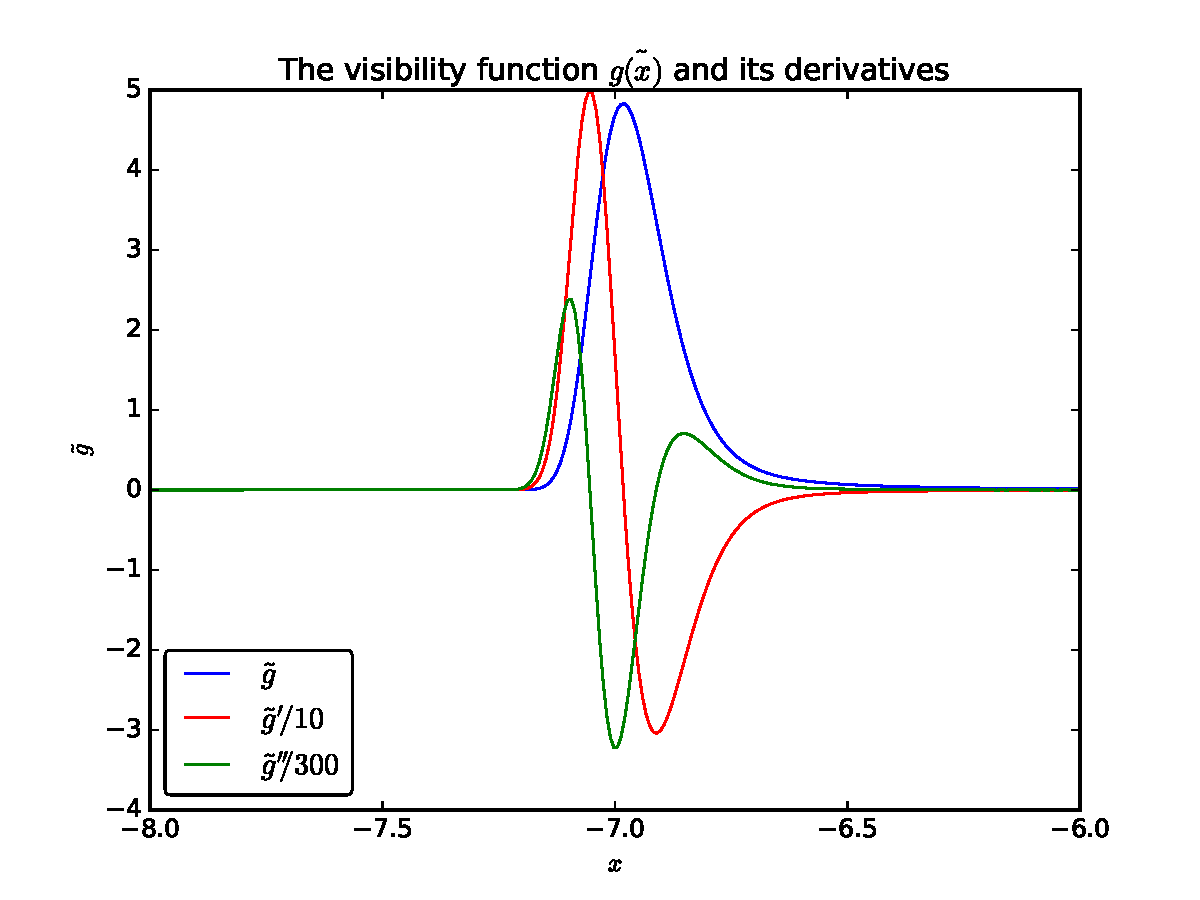
\includegraphics[width=\linewidth]{Plots/VisibilityFunc.pdf}
\caption{Plot of the visibility function $\tilde{g}(x)$ and its interpolated (and scaled) derivatives. We note the peak of the visibility function around the point $x=-7$. }
\end{figure}

\newpage
\FloatBarrier
\subsection*{The code}
\begin{lstlisting}
import numpy as np
import matplotlib.pyplot as plt
from scipy import interpolate
from scipy import integrate

# Global constants
# Units
eV = 1.60217647e-19
Mpc = 3.08568025e22

# Cosmological parameters
Omega_b = 0.046
Omega_m = 0.224
Omega_r = 8.3e-5
Omega_nu = 0.0
Omega_lambda = 1.0 - Omega_m - Omega_b - Omega_r - Omega_nu
T_0 = 2.725
n_s = 1.0
A_s = 1.0
h0 = 0.7
H_0 = h0*100.0*1e3/Mpc

# General constants
c = 2.99792458e8
epsilon_0 = 13.605698*eV
m_e = 9.10938188e-31
m_H = 1.673534e-27
sigma_T = 6.652462e-29
G_grav = 6.67258e-11
rho_c0 = (3.0*H_0**2)/(8*np.pi*G_grav)
alpha = 7.29735308e-3
hbar = 1.05457148e-34
k_b = 1.3806503e-23

# Density Parameters today
rho_m0 = Omega_m*rho_c0
rho_b0 = Omega_b*rho_c0
rho_r0 = Omega_r*rho_c0
rho_lambda0 = Omega_lambda*rho_c0

# Precalculate certain factors to reduce number of float point operations
Saha_b_factor = ((m_e*T_0*k_b)/(2*np.pi*hbar**2))**(3.0/2.0)		# Factor in front of 'b' in Saha equation
rhoCrit_factor = 3.0/(8*np.pi*G_grav)							# Used for critical density at arbitrary times

# Constant used for Peebles equation and some constant factors that can be precalculated
Lambda_2sto1s = 8.227
alpha_factor = ((64.0*np.pi)/(np.sqrt(27.0*np.pi)))*((alpha/m_e)**2.0)*(hbar**2.0/c)
beta_factor = (((m_e*T_0*k_b)/(2.0*np.pi))**(3.0/2.0))*(1.0/hbar**3.0)
Lambda_alpha_factor = ((3.0*epsilon_0/(hbar*c))**3.0)/(8*np.pi)**2.0
EpsTemp_factor = epsilon_0/(k_b*T_0)

class time_mod():
	def __init__(self, savefig):
		self.savefig = savefig		# If savefig = 0, plots the data. If savefig = 1, saves the plots in a pdf

		if savefig != 0 and savefig != 1:
			print 'Current value of savefig = ', savefig
			raise ValueError('Argument savefig not properly set. Try savefig = 1 (saves as pdf) or savefig = 0 (do not save as pdf)')

		self.n1 = 200
		self.n2 = 300
		self.n_t = self.n1 + self.n2

		self.z_start_rec = 1630.4
		self.z_end_rec = 614.2
		self.z_0 = 0.0
		self.x_start_rec = -np.log(1.0 + self.z_start_rec)
		self.x_end_rec = -np.log(1.0 + self.z_end_rec)
		self.x_0 = 0.0
		self.a_start_rec = 1.0/(1.0 + self.z_start_rec)
		self.a_end_rec = 1.0/(1.0 + self.z_end_rec)

		# Used for the x-values for the conformal time
		self.n_eta = 3000
		self.a_init = 1e-10
		self.x_eta_init = np.log(self.a_init)
		self.x_eta_end = 0

		# Set up grid, these are currently unused
		x_t_rec = np.linspace(self.x_start_rec, self.x_end_rec, self.n1)
		x_t_today = np.linspace(self.x_end_rec, self.x_0, self.n2)
		a_t_rec = np.linspace(self.a_start_rec, self.a_end_rec, self.n1)
		a_t_today = np.linspace(self.a_end_rec, 1, self.n2)
		# Merging the arrays into one
		self.x_t = np.concatenate([x_t_rec, x_t_today])
		self.a_t = np.concatenate([a_t_rec, a_t_today])

		# Set up grid of x-values for the integrated eta and tau
		self.x_eta = np.linspace(self.x_eta_init, self.x_eta_end, self.n_eta)	# X-values for the conformal time
		self.x_tau = np.linspace(self.x_eta_end, self.x_eta_init, self.n_eta)	# Reversed array, used to calculate tau

	def Get_Hubble_param(self, x):
		""" Function returns the Hubble parameter for a given x """
		return H_0*np.sqrt((Omega_b + Omega_m)*np.exp(-3*x) + Omega_r*np.exp(-4*x) + Omega_lambda)

	def Get_Hubble_prime(self, x):
		""" Function returns the scaled Hubble parameter for a given x value. See report 1 """
		return H_0*np.sqrt((Omega_b + Omega_m)*np.exp(-x) + Omega_r*np.exp(-2*x) + Omega_lambda*np.exp(2*x))

	def Get_Hubble_prime_derivative(self, x):
		""" Function returns the derivative of the scaled Hubble parameter. See report 1 """
		return -H_0**2*(0.5*(Omega_b + Omega_m)*np.exp(-x) + Omega_r*np.exp(-2*x) - Omega_lambda*np.exp(2*x))/(Get_Hubble_prime(x))

	def Get_Omegas(self, x):
		""" 
		Calculates the omegas as a function of redshift
		Will first have to calculate the energy densities today, which is then used to calculate the energy density
		for an arbitrary time. See report 1
		"""
		H = self.Get_Hubble_param(x)
		rho_c = rhoCrit_factor*H**2
		Omega_m_z = rho_m0*np.exp(-3*x)/rho_c
		Omega_b_z = rho_b0*np.exp(-3*x)/rho_c
		Omega_r_z = rho_r0*np.exp(-4*x)/rho_c
		Omega_lambda_z = rho_lambda0/rho_c

		return Omega_m_z, Omega_b_z, Omega_r_z, Omega_lambda_z

	def Diff_eq_eta(self, eta, x_0):
		""" Returns the right hand side of the differential equation for the conformal time eta """
		dEtada = c/(self.Get_Hubble_prime(x_0))
		return dEtada

	def Cubic_Spline(self, x_values, y_values, n_points, x_start=np.log(1e-10), x_end=0):
		""" 
		Cubic spline interpolation, zeroth derivative. Returns interpolated values of any variables, for a given range of x-values
		"""
		Temp_interp = interpolate.splrep(x_values, y_values)
		x_new = np.linspace(x_start, x_end, n_points)
		y_new = interpolate.splev(x_new, Temp_interp, der=0)
		return x_new, y_new

	def Spline_Derivative(self, x_values, y_values, n_points, derivative, x_start=np.log(1e-10), x_end=0):
		""" Spline derivative for any functions. Using natural spline """
		if derivative < 1:
			raise ValueError("Derivative input in Spline_Derivative less than 1. Use Cubic_spline instead.")
		Temp_interp = interpolate.splrep(x_values, y_values)
		x_new = np.linspace(x_start, x_end, n_points)
		yDerivative = interpolate.splev(x_new, Temp_interp, der=derivative)
		yDerivative[0] = 0
		yDerivative[-1] = 0
		return yDerivative

	def Get_Index_Interpolation(self, X_init, X_end):
		""" 
		Finds the array index/component of x for a given x-value
		This is specifically used to zoom into the interpolated segment
		"""
		EtaIndex1 = (np.abs(self.x_eta - X_init)).argmin()
		EtaIndex2 = (np.abs(self.x_eta - X_end)).argmin()
		if EtaIndex1-1 <= 0:
			EtaIndex1 = 0
		else:
			EtaIndex1 -= 1

		if EtaIndex2+1 >= self.n_eta:
			EtaIndex2 = self.n_eta-1
		else:
			EtaIndex2 += 1

		return EtaIndex1, EtaIndex2

	def Get_n_b(self, x):
		""" Calculate n_b (or n_H) at a given 'time' x """
		n_b = Omega_b*rho_c0*np.exp(-3.0*x)/m_H
		return n_b

	def Saha_equation(self, x):
		""" 
		Solves the Saha equation. Uses numpy.roots solver, see report. Only returns the positive valued X_e 
		"""
		Exponential = np.exp(x)
		a = 1
		b = (Saha_b_factor/self.Get_n_b(x))*np.exp(-EpsTemp_factor*Exponential - 3.0*x/2.0)
		c = -b
		X_e = np.roots(np.array([a,b,c]))

		if X_e[0] > 0:
			return X_e[0]
		else:
			return X_e[1]
		
	def Peebles_equation(self, X_e, x_0):
		""" Solves the right hand side of the Peebles equation """
		n_b = self.Get_n_b(x_0)
		H = self.Get_Hubble_param(x_0)
		exp_factor = EpsTemp_factor*np.exp(x_0)
		phi2 = 0.448*np.log(exp_factor)
		alpha2 = alpha_factor*np.sqrt(exp_factor)*phi2
		beta = alpha2*beta_factor*np.exp(-3.0*x_0/2.0-exp_factor)
		beta2 = alpha2*beta_factor*np.exp(-3.0*x_0/2.0-exp_factor/4.0)
		Lambda_alpha = H*Lambda_alpha_factor/((1.0-X_e)*n_b)
		C_r = (Lambda_2sto1s + Lambda_alpha)/(Lambda_2sto1s + Lambda_alpha + beta2)
		dXedx = (C_r/H)*(beta*(1.0-X_e) - n_b*alpha2*X_e**2.0)
		return dXedx

	def Calculate_Xe(self):
		""" Function that calculates X_e. Initial condition X_e = 1 """
		X_e_TempArray = [1]
		for i in range(0,self.n_eta-1):
			if X_e_TempArray[i] > 0.99:
				X_e_TempArray.append(self.Saha_equation(self.x_eta[i]))
			else:
				PeebleXe = integrate.odeint(self.Peebles_equation, X_e_TempArray[i], self.x_eta[i:])
				break

		PeebleXe2 = []
		for i in range(0, len(PeebleXe)-1):
			PeebleXe2.append(PeebleXe[i][0])
		self.X_e_array = np.concatenate([np.array(X_e_TempArray),np.array(PeebleXe2)])	# Merges arrays

	def Diff_eq_tau(self, tau, x_0):
		""" 
		Solves the differential equation of tau. This is the right hand side of the equation
		Finds the n_e value that corresponds to the x value, since we use a reversed x-array.
		"""
		i = np.searchsorted(self.x_eta, x_0, side="left")
		dTaudx = - self.n_e[i]*sigma_T*c/self.Get_Hubble_param(x_0)
		return dTaudx

	def Visibility_func(self, x, tau, tauDerv):
		""" Computes the visibility function (tilde) """
		g = np.zeros(len(tau))
		for i in range(0, len(tau)-1):
			g[i] = -tauDerv[i]*np.exp(-tau[i])
		return g
		
	def Plot_results(self, n_interp_points, x_start0 = -np.log(1.0 + 1630.4), x_end0 = -np.log(1.0 + 614.2)):
		""" Solves and plots the results """
		self.ScipyEta = integrate.odeint(self.Diff_eq_eta, 0, self.x_eta)
		# Calculate X_e, and n_e
		self.Calculate_Xe()
		self.n_e = self.X_e_array*self.Get_n_b(self.x_eta)
		# Calculates tau and interpolates the first and second derivatives
		Taus = integrate.odeint(self.Diff_eq_tau, 0, self.x_tau)[::-1]	# Calculate tau and reverse array
		TauDerivative = self.Spline_Derivative(self.x_eta, Taus, self.n_eta, derivative=1)
		TauDoubleDer = self.Spline_Derivative(self.x_eta, Taus, 200, derivative=2)
		# Calculate g, and interpolates the first and second derivatives
		g_tilde = self.Visibility_func(self.x_eta, Taus, TauDerivative)
		g_tildeDerivative = self.Spline_Derivative(self.x_eta, g_tilde, self.n_eta, derivative=1)
		g_tildeDoubleDer = self.Spline_Derivative(self.x_eta, g_tilde, self.n_eta, derivative=2)
		
		fig1 = plt.figure()
		ax1 = plt.subplot(111)
		ax1.semilogy(self.x_eta, self.X_e_array)
		ax1.set_ylim([10**(-4), 1.3])
		plt.xlabel('$x$')
		plt.ylabel('$X_e$')
		plt.title('Number of free electrons $X_e$ as a function of $x=\ln(a)$')

		fig2 = plt.figure()
		ax2 = plt.subplot(111)
		ax2.semilogy(self.x_eta, self.X_e_array)
		ax2.set_ylim([10**(-4), 1.3])
		ax2.set_xlim([-7.5, -5])
		plt.xlabel('$x$')
		plt.ylabel('$X_e$')
		plt.title('Number of free electrons $X_e$, zoomed in')
		
		fig3 = plt.figure()
		ax3 = plt.subplot(111)
		plt.hold("on")
		ax3.semilogy(self.x_eta, Taus, 'b-', label=r'Zeroth derivative $\tau$')
		ax3.semilogy(self.x_eta, np.fabs(TauDerivative), 'r-', label=r"First derivative $|\tau'|$")
		ax3.semilogy(np.linspace(self.x_eta_init, self.x_eta_end, 200), np.fabs(TauDoubleDer), 'g-', label=r"Second derivative $|\tau''|$")
		plt.xlabel('$x$')
		plt.ylabel('$n_e$')
		plt.title(r"Plot of $\tau$ and $|\tau'|$ as a function of $x=\ln(a)$")
		ax3.legend(loc='upper right', bbox_to_anchor=(1,1), ncol=1, fancybox=True)
		
		fig4 = plt.figure()
		ax4 = plt.subplot(111)
		plt.hold("on")
		ax4.plot(self.x_eta, g_tilde, 'b-', label=r"$\tilde{g}$")
		ax4.plot(self.x_eta, g_tildeDerivative/10.0, 'r-', label=r"$\tilde{g}'/10$")
		ax4.plot(self.x_eta, g_tildeDoubleDer/300.0, 'g-', label=r"$\tilde{g}''/300$")
		ax4.set_xlim([-8,-6])
		plt.xlabel('$x$')
		plt.ylabel(r'$\tilde{g}$')
		plt.title(r"The visibility function $\tilde{g(x)}$ and its derivatives")
		ax4.legend(loc='lower left', bbox_to_anchor=(0,0), ncol=1, fancybox=True)
		
		if self.savefig == 1:
			fig1.savefig('../Plots/ElectronNumber.pdf')
			fig2.savefig('../Plots/ElectronNumberZoomed.pdf')
			fig3.savefig('../Plots/FirstDerivativeTau.pdf')
			fig4.savefig('../Plots/VisibilityFunc.pdf')
		else:
			plt.show()

solver = time_mod(savefig=1)
solver.Plot_results(100)
\end{lstlisting}

\begin{thebibliography}{1}
    \bibitem{cpyhsics} P. Callin, \url{https://arxiv.org/abs/astro-ph/0606683}.
\end{thebibliography}
\end{document}